\begin{table}[h]
\begin{tabular}{ccc}
\hline \\
Matrix & Schaltung & Wahrheitstabelle \\
\hline \\

\begin{equation} X = \begin{bmatrix} 0 & 1 \\ 1 & 0 \end{bmatrix} \end{equation} &
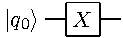
\includegraphics[width=0.2\textwidth]{figures/pauli_x.pdf} &
\begin{tabular}{|c||c||c|}
\hline
Fall & $q_0$ & $X|q_0\rangle$ \\
\hline\hline
1 & $|0\rangle$ & $|1\rangle$ \\
0 & $|1\rangle$ & $|0\rangle$ \\
\hline
\end{tabular} \\

\begin{equation} Y &= \begin{bmatrix} 0 & -i \\ i & 0 \end{bmatrix}\end{equation} &
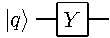
\includegraphics[width=0.2\textwidth]{figures/pauli_y.pdf} &
\begin{tabular}{|c||c||c|}
\hline
Fall & $q_0$ & $X|q_0\rangle$ \\
\hline\hline
1 & $|0\rangle$ & $i|1\rangle$ \\
0 & $|1\rangle$ & $-|1\rangle$ \\
\hline
\end{tabular}


\end{tabular}
\end{table}
